\documentclass{IEEEtran}
\usepackage[utf8]{inputenc}
\usepackage[T1]{fontenc}
\usepackage[ngerman]{babel}
\usepackage[nolist]{acronym}
\usepackage{footnote}
\usepackage{algorithmic}
\usepackage{graphicx}
\usepackage[autostyle=true,german=quotes]{csquotes}
\usepackage{gensymb}
\usepackage{eurosym}
\usepackage{booktabs}
\usepackage{array}
\usepackage{todonotes}
\usepackage{microtype}
\usepackage{icomma}


\usepackage{hyperref}

\long\def\comment / *#1* /{}



% -----------------------------------------------------------------------------
% Visible TODO and FIXME markers
% -----------------------------------------------------------------------------
\newcounter{TODOCOUNT}
\newcommand{\TODO}[1]{\vspace{0.5em}\todo[inline, color=orange]{#1}\stepcounter{TODOCOUNT}}
\newcommand{\FIXME}[1]{\todo[size=\small, color=red]{#1}\stepcounter{TODOCOUNT}}
\AtEndDocument{
	\ifnum\value{TODOCOUNT}>0
		%\cleardoublepage
		\listoftodos
	\fi
}
% -----------------------------------------------------------------------------


\newcolumntype{x}[1]{>{\centering\arraybackslash\hspace{0pt}}p{#1}}



\begin{document}


\title{cowbusconfig -- Ansatz zur dezentralen Konfiguration von Gebäudeautomation}
\author{Patrick~Kanzler \and Michael~Zapf}
\date{\today}



\maketitle

\todo{nochmal über die Abkürzungen drüber gehen und schauen, wo man schön abkürzt (wenn der Text steht.)}

\begin{abstract}
    Um die Vorzüge intelligenter Haussteuerung einer breiten Masse zugänglich
    zu machen, müssen die System einfach handhabbar werden.
    Besonders die Konfiguration, also die Zuordnung von Sensorevent zu
    Schaltaktion, muss einfach durchführbar und ebenso einfach anpassbar
    bzw. revidierbar sein. Diese Arbeit schlägt einen Ansatz vor,
    der in einem dezentralen Sensor-Aktor-Netzwerk eine einfache
    Konfigurationsmöglichkeit bieten soll.
    Dabei erfolgt die eigentliche Konfiguration per Webbrowser und kann
    jederzeit wieder ausgelesen, geändert und ergänzt werden.
\end{abstract}

\section{Einleitung}
    \enquote{Smart Home} ist ein Schlagwort, um das man im 21. Jahrhundert
    kaum noch herum kommt. Der moderne Mensch möchte sein Zuhause vernetzen.
    Vor allem in gewerblich genutzten Gebäuden ist es inzwischen üblich,
    auf die in der Vergangenheit übliche harte Verdrahtung von Sensoren und
    Aktoren -- sprich zum Beispiel Lichtschalter und Leuchte -- zu verzichten
    und auf intelligente Einzelkomponenten zu setzen, die meist in einer
    Bustopologie verbunden sind. Der Vorteil liegt auf der Hand:
    Durch das Fehlen der festen und starren Zuordnung zwischen auslösendem
    Ereignis (\emph{Lichtschalter gedrückt}) und Wirkung (\emph{Leuchte A an})
    können softwarebasiert Ursache-Wirkung-Beziehungen modelliert, evaluiert
    und korrigiert werden.

    Etablierte Systeme setzen dabei in der Regel auf eine
    Konfigurationssoftware, in der die teils komplexen Kommunikation- und
    Schaltvorgänge modelliert werden.
    Die einzelnen an den Bus angeschlossenen Komponenten werden häufig nur
    mit dem logischen Endergebnis konfiguriert,
    aus dem sich die ursprünglichen Absichten nicht mehr vollständig ableiten
    lassen.

    In dieser Arbeit beschäftigen wir uns mit dem Gedanken,
    Teilnehmer in einem Gebäudeautomationsnetzwerk so konfigurierbar zu gestalten,
    dass die Konfiguration jederzeit mit minimalen Aufwand auslesbar
    und änderbar ist.
    Die Idee ist im Kontext der Vorlesung zum Thema \ac{DIY} von Dr.-Ing. Jürgen Eckert als studentisches
    Projekt entstanden und zielt deshalb auch einfachste Anforderungen ab.

\section{Verwandte Arbeiten}
    Gebäudeautomation wird inzwischen sowohl in der Praxis
    als auch in der Forschung erprobt. Hierbei konkurrieren verschiedene Systeme
    und Technologien, denen unterschiedlichste Paradigmen zugrunde liegen.
    Zur Veranschaulichung möchten wir hier ein System aus der Praxis betrachten,
    das auf dezentraler Kommunikation beruht,
    sowie einen Ansatz aus der Forschung,
    der einen zentralen Kommunikationsserver vorschlägt.

    \subsection{Europäischer Installationsbus (EIB) / KNX}
    Der unter der Abkürzung EIB bekannte Europäische Installationsbus
    ist ein offener Standard und nach subjektivem Empfinden das in der Praxis
    wohl meistgenutzte System in der Gebäudeautomation.
    Inzwischen wird er unter dem Namen KNX entwickelt und vertrieben.
    Es sind weltweit fast 7000 Produkte auf dem Markt\footnote{ KNX Association, \enquote{KNX -- Technologie -- Einführung}, \url{http://www.knx.org/knx-de/knx/technologie/einfuehrung/index.php}},
    die mit einer Twisted-Pair-Leitung verbunden werden
    (weitere Medien -- auch drahtlose -- sind verfügbar),
    über die Nachrichten direkt untereinander ausgetauscht werden\footnote{KNX Association, \enquote{KNX -- Technologie -- Kommunikationsmedien}, \url{http://
www.knx.org/knx-de/knx/technologie/kommunikationsmedien/index.php}}.

    Die Konfiguration der Schaltregeln etc. erfolgt nach der Installation
    der Komponenten durch einen Fachmann mithilfe von Software aus der
    ETS-Familie. Dabei handelt es sich um proprietäre Software,
    die von der KNX Association\footnote{KNX Association, \enquote{KNX System Specifications -- Architecture}, 2001}
    entwickelt und vertrieben wird.
    \todo{Platzierung der Fußnoten optimieren}
    

    KNX eignet sich besonders im Bereich großer Gebäude, in denen die
    elektrischen Systeme von einem Fachmann geplant, installiert und auch über
    Jahre hinweg gewartet werden. Ein entscheidender Nachteil von KNX ist,
    dass die Konfiguration, sobald sie einmal in die Steuergeräte geschrieben
    ist, nicht mehr ohne weiteres ausgelesen werden kann.
    Um die Konfiguration zu ändern (um zum Beispiel neue Komponenten einzufügen
    oder auch nur eine einfache Schaltregel anzupassen) wird jedes mal
    die ursprünglich erstellte Projektdatei aus der ETS-Software benötigt.

    \subsection{Zentrale skriptbasierte Steuerung}
        T. Haenselmann et al. \cite{haenselmann2007skriptbasierte}
        beschreiben ein zentrales System, das weitgehend
        unabhängig von dem verwendeten Transportmedium ist.
        Sie schlagen eine drahtlose Kommunikation vor,
        der Kerngedanke jedoch, auf den wir uns hier beziehen werden,
        gilt jedoch medienunabhängig.
        Der grundlegende Ansatz besteht in der Einrichtung eines zentralen
        Servers, bei dem alle Nachrichten des Systems zusammenlaufen.
        Sensoren melden ihre Messwerte an diesen, der dann Schaltnachrichten
        an die Aktoren sendet.
        Die Entscheidung, welche Aktionen ausgelöst werden, trifft der Server
        mithilfe von Skripten, die der Benutzer hinterlegt.
        Diese Skripte können auch über eine Weboberfläche erstellt und
        verwaltet werden.

    %\cite{drossos2013ansteuerung}
    %\cite{kuntz6servicecast}
    %\cite{kuntz2011dienstbasierte}

\section{Ansatz}
    Inspiriert von Haenselmann et al. \cite{haenselmann2007skriptbasierte}
    möchten wir ein System vorschlagen,
    das ebenso über eine einfache Weboberfläche konfiguriert werden kann.
    Der Benutzer kann dort einfache Wenn-Dann-Regeln anlegen, bearbeiten und
    löschen, die das Verhalten der Aktoren in Abhängigkeit von Sensorereignissen
    festlegen.

    Der grundlegende Unterschied im Ansatz besteht jedoch darin,
    dass wir auf eine zentrale Kommunikationseinheit verzichten.

    \subsection{Voraussetzungen, Annahmen}
        Wir gehen davon aus, dass uns ein paketvermitteltes Netz vorliegt,
        in dem alle Teilnehmer eindeutig adressierbar sind.

        Als Test- und Referenzumgebung dient uns der \emph{cowbus}.
        Dabei handelt es sich um ein studentisches Projekt,
        das sich zum Ziel gesetzt hat,
        eine kostengünstige und einfach nachzubauende Plattform zu schaffen,
        die einen Einstieg in den Arbeits- und Forschungsbereich des
        \enquote{Smart Home} bzw. \enquote{Connected Home} ermöglichen soll.
        Der Nachrichtenaustausch erfolgt dabei drahtlos über eine
        $2,4$\,GHz-Funkverbindung. Eine umfangreichere Beschreibung des Projektes
        steht auf der
        Projektseite\footnote{\url{http://www7.cs.fau.de/de/wp-content/uploads/sites/2/2014/08/projektdoku_cowbus.pdf}}
        des Lehrstuhles zur Verfügung.
        \todo{Github-Seite unterbringen}

        Das Testnetzwerk besteht aus drei Komponenten:
        \begin{itemize}
            \item Als \textbf{Sensor} dient ein einfacher Taster.
                Er soll Schaltaktionen im Netzwerk auslösen.
            \item Eine LED dient als \textbf{Aktor},
                der beliebige Schaltaktionen im Netzwerk symbolisch darstellt.
            \item Zur \textbf{Konfiguration} der Geräte befindet sich
                außerdem ein zusätzlicher Computer im Netzwerk.
                In unserem Aufbau haben wir dafür einen Raspberry Pi gewählt.
                Er wurde um ein Funkmodul erweitert und stellt eine
                Weboberfläche zur Verfügung,
                über die die Konfiguration ermöglicht werden soll.
                Außerdem ermöglicht er die \textbf{Überwachung} des Netzwerkverkehrs.
        \end{itemize}

    \subsection{Idee}
        Da \textbf{Sensoren} häufig höhere Anforderungen an den Energieverbrauch
        stellen, sollen sie in dem System \enquote{dumm} sein.
        Sie erarbeiten sich also kein Wissen über die anderen Netzwerkkomponenten
        und reagieren nicht, sondern agieren ausschließlich.
        Das ermöglicht uns sie die meiste Zeit in Energiesparmodi zu betreiben
        und nur dann aufzuwecken, wenn sie selbst ein Ereignis auslösen,
        zum Beispiel wenn der Benutzer einen Taster betätigt.

        \textbf{Aktoren} hingegen sind häufig mit stabilen Energiequellen
        ausgestattet, da sie meist gewisse Lasten schalten.
        Als Beispiele wären Leuchten, Jalousiemotoren oder auch Ventilatoren
        zu nennen.
        Daher bietet es sich an, logische Verknüpfungen hier vorzunehmen.

        Die \textbf{Konfiguration} der Aktoren wird über ein webfähiges Gerät
        vorgenommen, das über ein herkömmliches \ac{LAN} die
        Konfigurationswebseite des Raspberry Pi anzeigt.
        Dabei werden Konfigurationsnachrichten quasi \enquote{in-band}
        über den Funkkanal gesendet.
        Die Aktoren erkennen sie an den speziellen Nachrichtentypen.

    \subsection{Regeln}
        Basis der Logik sind sind einfache Wenn-Dann-Regeln.
        Ein (Aktor)-Knoten kann theoretisch beliebig viele dieser Regeln befolgen.

        Eine Regel besteht aus mehreren Komponenten.
        Zur Veranschaulichung wird jede Komponente am Beispiel unserer
        Testumgebung erklärt: Der Schalter soll die Lampe an- bzw. abschalten.
        \begin{enumerate}
            \item Festgelegt wird, auf Pakete welcher \textbf{Adresse}
                die Regel zutrifft.
                Im Beispiel wäre dies die Adresse des Schalters.
            \item Die \textbf{Operator} legt fest, wie der angegebene
                Schwellwert der Regel mit dem im Paket übertragenen Wert
                verglichen wird.
                Im Schalter-Lampe-Beispiel bietet sich hier der Test auf Gleichheit an.
            \item Verglichen wird jeweils mit dem bereits erwähnten
                \textbf{Schwellwert}. Wenn als Operator eine Intervallprüfung
                gewählt wird, müssen zwei Schwellwerte
                (ein oberer und ein unterer) angegeben werden.
                Im Beispiel sind hier die Werte 0 für \enquote{an}
                und 1 für \enquote{aus} sinnvoll.
            \item Die \textbf{Aktion} gibt an, was der Aktor macht,
                wenn ein Paket eingetroffen ist, auf das die Regel zutrifft.
        \end{enumerate}

        %Unter der Annahme, dass der Schalter im Zustand \enquote{an} eine
        %\enquote{1} und im Zustand \enquote{aus} eine \enquote{0} sendet
        %ergeben sich also zwei Regeln:

		\todo{Das Beispiel muss angepasst werden, sodass es einheitlich ist. + ERKLÄRUNG}
        

        Soll ein Ventilator aktiviert werden, wenn der Wert eines Temperatursensors
        im Intervall $[18;25]$ liegt, könnten die zugehörigen Regeln wie folgt aussehen:

        \begin{center}
            \begin{tabular}{r|x{0.15\textwidth}|x{0.15\textwidth}}
                \toprule
                                        & \textbf{Regel 1} & \textbf{Regel 2} \\
                \midrule
                \textbf{Adresse}:       & \multicolumn{2}{c}{Sensoradresse} \\
                \textbf{Operator}:     & \enquote{$\leq \geq$} & \enquote{nicht $\leq \geq$} \\
                \textbf{Schwellwert A}: & \multicolumn{2}{c}{18} \\
                \textbf{Schwellwert B}: & \multicolumn{2}{c}{25} \\
                \textbf{Aktion}:        & \enquote{Ventilator an}  & \enquote{Ventilator aus} \\
                \bottomrule
            \end{tabular}
        \end{center}

    \subsection{Operator}
		In den cowbus-Knoten sind die grundlegenden logischen Operatoren implementiert.
		Damit lassen sich bereits die meisten Schaltaufgaben abbilden.
		\todo{Entweder ganz weg oder ausbauen.}
    \subsection{Konfigurationsnachrichten}
        Um die Konfiguration jederzeit auslesbar und änderbar zu gestalten
        sind folgende Nachrichtentypen vorgesehen:

        \begin{itemize}
            \item Erhält ein Knoten das Kommando \textbf{LIST} antwortet
                er mit Nachrichten des Typs \textbf{ANSWER\_LIST},
                die alle auf ihm gespeicherten Regeln enthalten.
            \item Eine Nachricht mit dem Kommando \textbf{ADD} weist einen
                Knoten an die in der Nachricht enthaltene Regel zu seiner
                Regelliste hinzuzufügen und in Zukunft zu beachten.
            \item Eine bestimmte Regel kann von einem Knoten gelöscht werden,
                indem man ihm eine Nachricht mit dem Kommando
                \textbf{DELETE\_ONE} sendet, die eine auf dem Knoten eindeutige
                laufende Nummer der Regel enthält.
                (Die laufenden Nummern der Regeln können mit dem
                \emph{LIST}-Kommando abgefragt werden.)
            \item Mit dem Kommando \textbf{DELETE\_ALL} kann die Konfiguration
                eines Knotens vollständig zurückgesetzt werden.
            \item Das Kommando \textbf{DELETE\_ADDR} weist einen Knoten an,
                alle Regeln mit einer bestimmten Adresse zu löschen,
                die in der Nachricht übertragen werden muss.
        \end{itemize}


\section{Evaluation}
    Der vorgestellte Ansatz funktioniert im kleinen Maßstab sehr gut.
    Besonders sehr einfache Schaltregeln lassen sich damit ohne großen Aufwand
    realisieren, zum Beispiel:
    \begin{itemize}
        \item \enquote{Schalter wurde auf \emph{AN} gestellt} $\Rightarrow$
            \enquote{Schalte Lampe an}
        \item \enquote{Temperatur übersteigt den Schwellwert von $28\degree$C} $\Rightarrow$
            \enquote{Schalte Ventilator an}
    \end{itemize}

    \TODO{Evaluation weiter? Positives?}

    Offen bleiben jedoch Fragen, wie komplexere logische Abhängigkeiten
    dargestellt werden können.
    Zu Beispiel wäre es unter Umständen interessant, eine Aktion nur auszuführen,
    wenn ein bestimmtes Ereignis über einen bestimmten Zeitraum mehrfach ohne
    widersprüchliche \enquote{Ausreißer} auftritt.
    So könnte es im Beispiel des Ventilators sinnvoll sein, diesen nur zu
    aktivieren, wenn der Temperaturwert über eine Minuten lang konstant über
    dem Schwellwert liegt, um versehentliche Schaltaktionen aufgrund von
    Messfehlern zu vermeiden, die sowieso wenige Sekunden später revidiert
    würden.

    In diesem Fall könnte auch eine Betrachtung der Tendenzen sinnvoll sein,
    also ob ein Messwert über die Zeit eher steigt oder fällt.
    Auch eine Mittelwertbildung könnte interessant sein.

    Ein möglicher Ansatz solche komplexeren Aufgaben zu realisieren,
    wäre einen Pseudo-Sensor-Aktor in das Netz zu setzen, der eingehende
    Ereignisse aufzeichnet, auswertet und dann unter bestimmten Bedingungen
    selbst ein Ereignis auslöst, sowie eben auch über die dafür benötigten
    Ressourcen verfügt. Ein solcher Knoten wäre dann entsprechend
    aufwändiger zu konfigurieren.


\section{Zusammenfassung und Ausblick}
    Mit cowbusconfig haben wir einen Ansatz zur einfachen Konfigurierbarkeit
    von Sensor-Aktor-Netzwerken im Hausautomationsbereich vorgestellt.
    Die Besonderheit gegenüber bisher üblichen oder erforschten Ansätzen ist
    dabei die Möglichkeit auf zentrale \enquote{Logik}-Komponenten
    zu verzichten und trotzdem die Konfiguration wiederauslesbar und
    änderbar zu gestalten.
    Damit ist es möglich, auf einfache Art und Weise neue Komponenten in das
    System zu integrieren und entsprechende Schaltregeln hinzuzufügen bzw.
    anzupassen, ohne das komplette System neu einstellen zu müssen.


        \begin{figure}
            \centering
            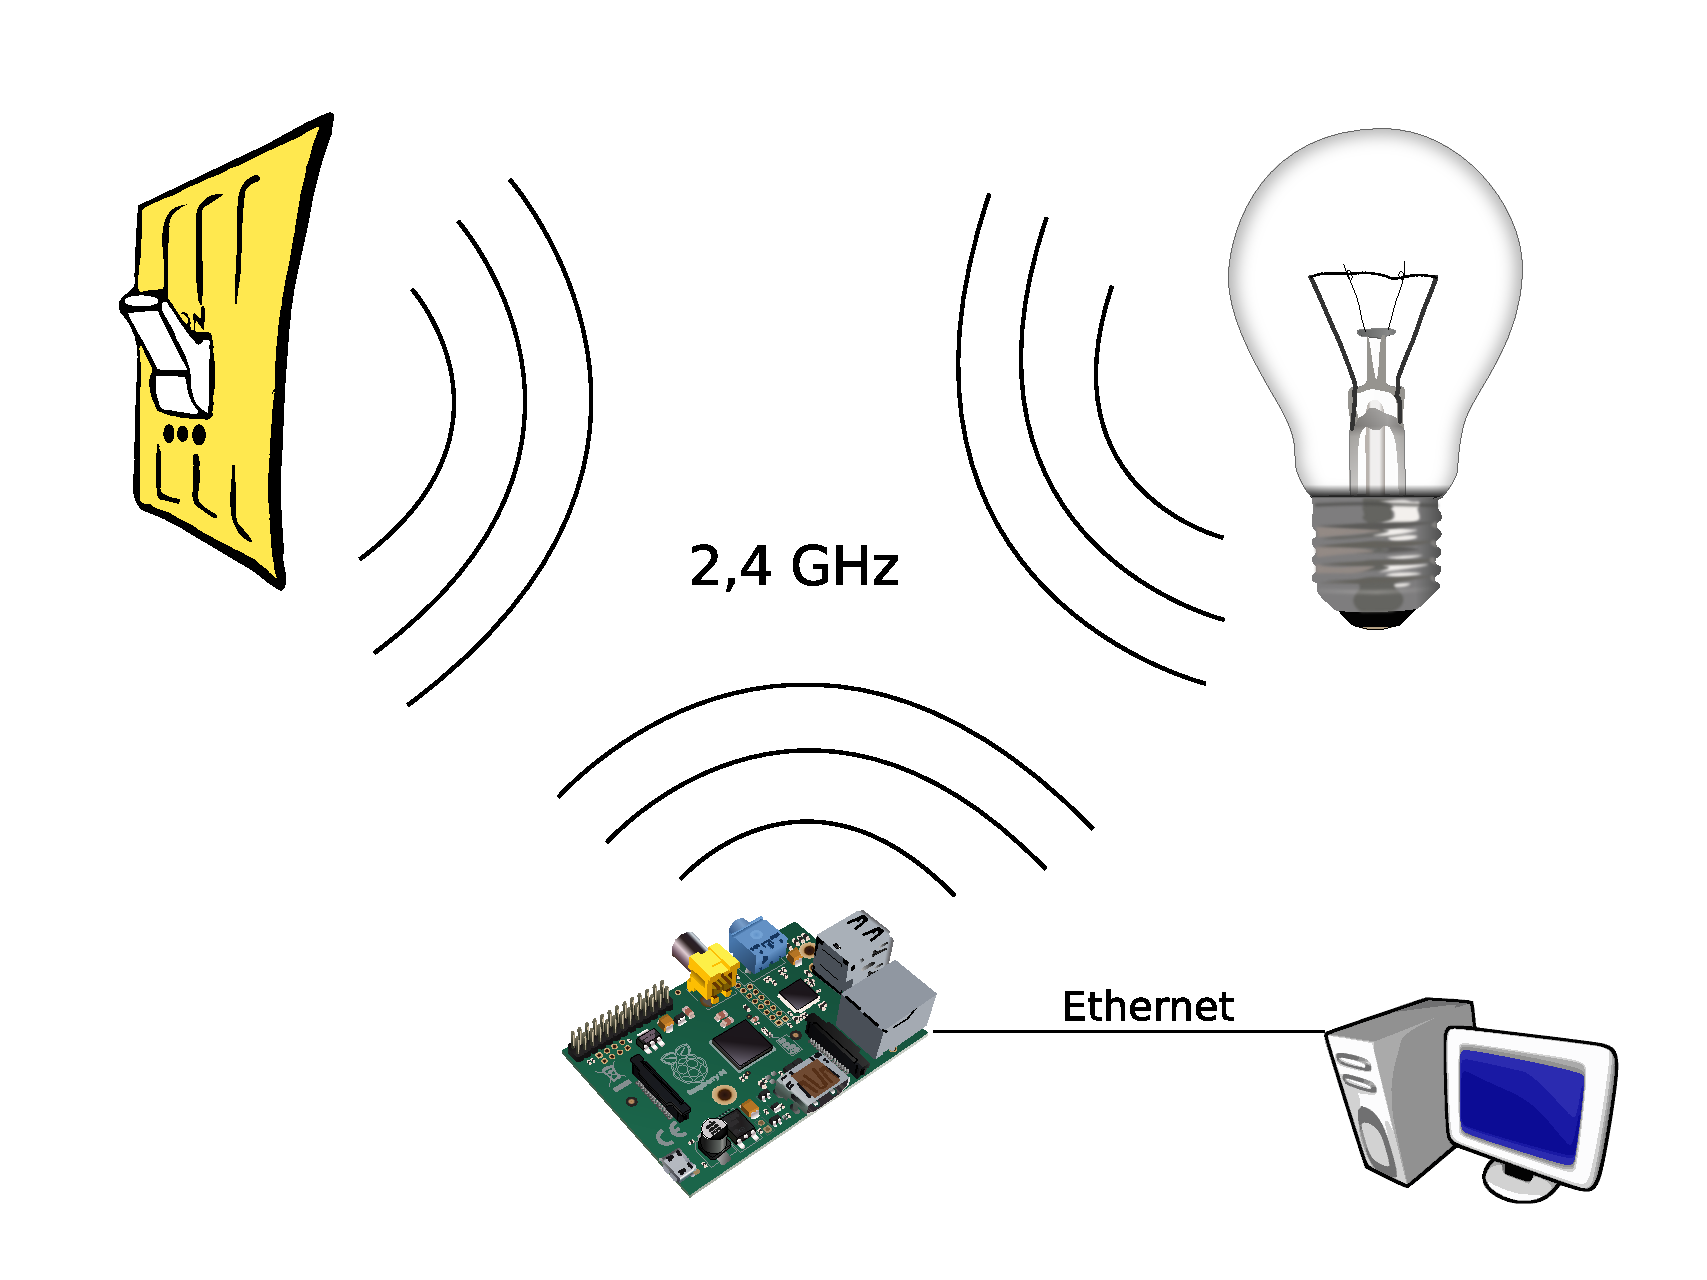
\includegraphics[width=0.5\textwidth]{img/system}
            \caption{Schematische Darstellung der Testumgebung}
            \label{fig:comp}
        \end{figure}


%\section*{Abkürzungen}
\renewcommand{\IEEEiedlistdecl}{\IEEEsetlabelwidth{CSMA/CA}}
\begin{acronym}
    \acro{DIY}{Do-It-Yourself}
    \acro{LAN}{Local Area Network}
\end{acronym}
\renewcommand{\IEEEiedlistdecl}{\relax}% remember to reset \IEEEiedlistdecl

\comment / *
\listoffigures
\clearpage

\listoftables
\clearpage
* /


\bibliographystyle{IEEEtran}
\bibliography{IEEEabrv,projektdoku_cowbus}

\end{document}
